\chapter{Casos de Uso}\label{apendice.A}
\section{Introducción}
\subsection{Propósito}
El propósito de este documento es describir de una forma clara y concreta cada uno de los casos de uso definidos para el sistema web a implementar.
\subsection{Alcance}
Los casos de uso presentados en este documento representan los requerimientos que se desean implementar en el sistema web para el aprendizaje colaborativo.
\subsection{Definiciones, acrónimos y abreviaciones}
\begin{enumerate}
  \item CU: Caso de uso
  \item SAC: Sistema para el aprendizaje colaborativo
\end{enumerate}
\clearpage
\section{Catálogo de actores}
En el la figura \ref{fig:actores} se puede ver los actores que participan en el SAC y en la Tabla \ref{tab:actores} se encuentra una breve descripción de cada uno de los actores.
\begin{figure}
  \centering
  % Requires \usepackage{graphicx}
  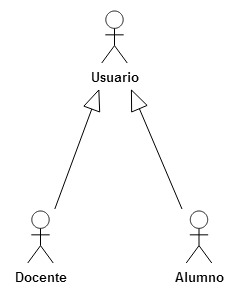
\includegraphics[scale=0.6]{figuras/casosdeuso/actores.jpg}\\
  \caption[Diagrama de actores]{Diagrama de actores}
  \label{fig:actores}
\end{figure}

\begin{longtable}{|L{3cm}|L{7cm}|}
\caption{Actores}
\label{tab:actores}\\
    \hline
    ACTOR & DESCRIPCIÓN \\
    \hline
    Usuario & Persona que usará el sistema web de tiempo real para el aprendizaje colaborativo.\\
    \hline
    Docente & Es la persona responsable de crear y dirigir las sesiones de clase que serán aplicadas a los alumnos. Además, el docente es el responsable de las evaluaciones que rendirán los alumnos una vez terminada cada sesión de clase.\\
    \hline
    Alumno & Es la persona que será instruida en temas de algoritmos y programación a través de cada sesión diseñada por el docente.\\
    \hline
\end{longtable}
\clearpage
\begin{landscape}
\section{Diagramas de casos de uso}
\subsection{Casos de uso}
\begin{figure}[!h]
  \centering
  % Requires \usepackage{graphicx}
  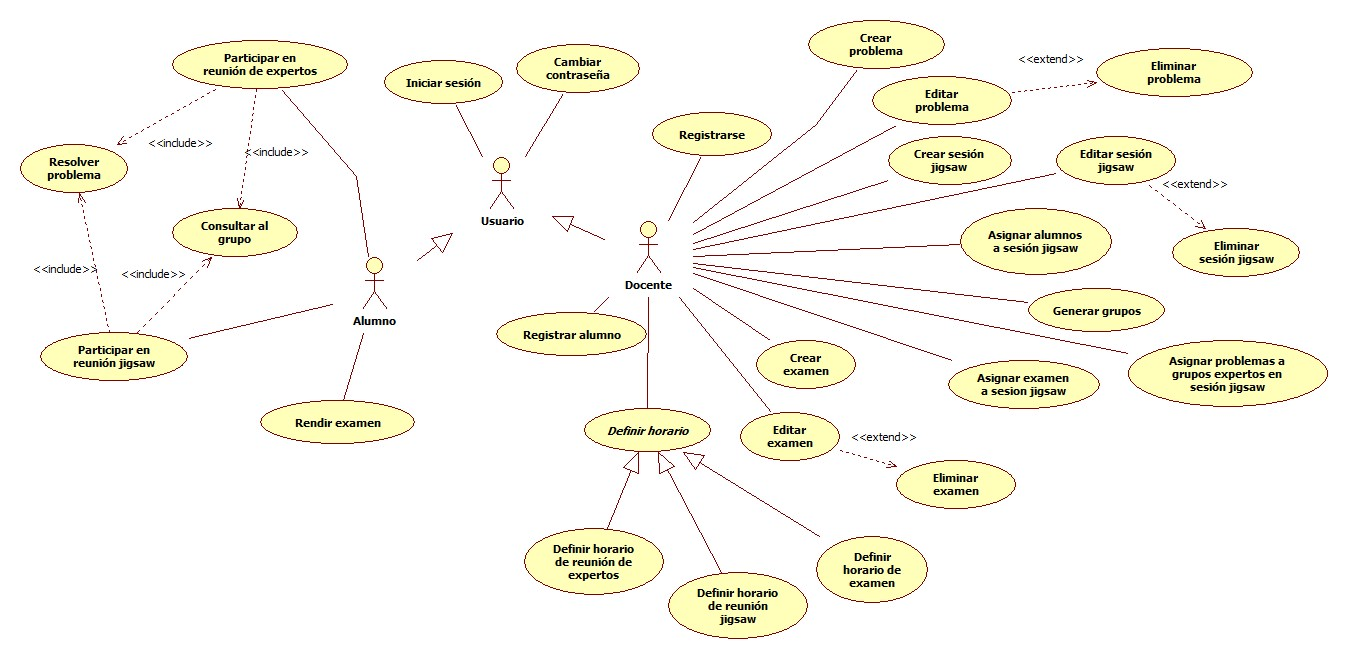
\includegraphics[scale=0.45]{figuras/casosdeuso/casos_de_uso.jpg}\\
  \caption[Casos de uso]{Diagrama de casos de uso para el sistema JigsawCoding}
  \label{fig:casos_de_uso}
\end{figure}
\end{landscape}
\clearpage
%\subsection{Casos de uso - Alumno}
%\begin{figure}[!h]
%  \centering
%  % Requires \usepackage{graphicx}
%  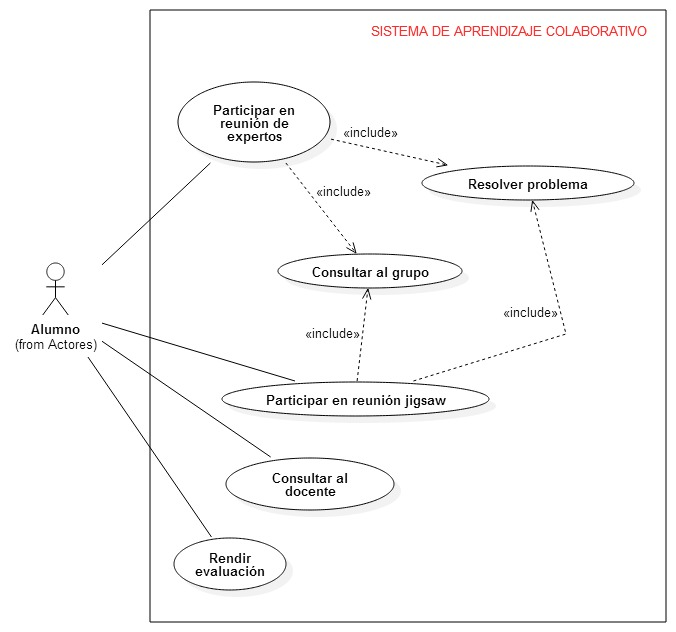
\includegraphics[scale=0.6]{figuras/casosdeuso/DCU_Alumno.jpg}\\
%  \caption[Casos de uso - Alumno]{Casos de uso - Alumno}
%  \label{fig:cus-alumno}
%\end{figure}
%\clearpage
\section{Especificaciones de Casos de Uso}
\subsection{Registrar Alumno}
\begin{longtable}{|c|L{10cm}|}
  \hline
  % after \\: \hline or \cline{col1-col2} \cline{col3-col4} ...
  Código &  CUS-\casodeuso\\  \hline
  Nombre &  REGISTRAR ALUMNO\\  \hline
  Descripción & El caso de uso inicia cuando el docente selecciona la opción registrar nuevo alumno. Luego completa la información del alumno y el caso de uso termina cuando se presiona la opción Guardar \\  \hline
  Actores & Docente \\  \hline
  Precondiciones &  El docente debe estar logueado en el sistema.\\  \hline
  Postcondiciones &  Ninguna\\  \hline
  Flujo básico &  \begin{enumerate}
                    \item El docente selecciona la opción para registrar un nuevo alumno.
                    \item El sistema muestra el formulario para completar los datos del alumno.
                    \item El docente completa los campos DNI, Apellido Paterno, Apellido Materno, Nombres, Email, Sexo, Email, Contraseña, Repetir Contraseña.
                    \item El sistema valida el formato del DNI, apellidos, nombres, email.
                    \item El sistema valida que el email no esté registrado en el sistema.
                    \item El sistema verificar que los campos contraseña y repetir contraseña sean idénticos.
                    \item El sistema registra al nuevo alumno en el sistema.
                  \end{enumerate}
  \\  \hline
  Flujo alternativo &  Ninguno\\  \hline
\end{longtable}
\clearpage
\subsection{Crear Problema}

%\begin{tabular}{|c|L{9cm}|}
%  \hline
%  % after \\: \hline or \cline{col1-col2} \cline{col3-col4} ...
%  Código &  CUS-\casodeuso\\  \hline
%  Nombre &  \\  \hline
%  Descripción &  \\  \hline
%  Actores &  \\  \hline
%  Precondiciones &  \\  \hline
%  Postcondiciones &  \\  \hline
%  Flujo básico &  \\  \hline
%  Flujo alternativo &  \\  \hline
%\end{tabular}

\begin{longtable}{|c|L{9cm}|}
  \hline
  % after \\: \hline or \cline{col1-col2} \cline{col3-col4} ...
  Código & CUS-\casodeuso \\  \hline
  Nombre & CREAR PROBLEMA \\  \hline
  Descripción & El caso de uso inicia cuando el usuario accede al sistema y elige la opción crear problema. Luego el usuario redacta el enunciado y demás observaciones sobre el problema y finaliza el caso de uso \\  \hline
  Actores & Docente \\  \hline
  Precondiciones & El usuario de ser un Docente y estar logueado en el sistema \\  \hline
  Postcondiciones & El docente verá en la lista de problemas el problema recién creado \\  \hline
  Flujo básico & \begin{enumerate}
                   \item El docente elige la opción NUEVO PROBLEMA
                   \item El sistema solicita al docente ingresar el título y enunciado del problema
                   \item El docente escribe el título y enunciado del problema
                   \item El docente selecciona la opción GUARDAR
                   \item El sistema guarda el nuevo problema
                 \end{enumerate}    \\  \hline
  Flujo alternativo & Ninguno \\  \hline
\end{longtable}
\clearpage
\subsection{Crear grupo experto}
\begin{longtable}{|c|L{9cm}|}
  \hline
  % after \\: \hline or \cline{col1-col2} \cline{col3-col4} ...
  Código &  CUS-\casodeuso\\  \hline
  Nombre &  CREAR GRUPO EXPERTO\\  \hline
  Descripción &  El caso de uso inicia cuando el usuario accede al sistema y elige la opción crear grupo experto. Luego completa la información sobre el grupo experto a crear y finalmente el caso de uso termina cuando el sistema crea experto.\\  \hline
  Actores &  Docente\\  \hline
  Precondiciones &  El usuario de ser un Docente y estar logueado en el sistema.\\  \hline
  Postcondiciones &  El docente verá en el listado de grupos expertos el nuevo grupo creado\\  \hline
  Flujo básico &    \begin{enumerate}
                        \item El docente elige la opción NUEVO GRUPO EXPERTO.
                        \item El docente digita el nombre para el grupo experto
                        \item El docente indica el máximo de integrantes que se pueden incluir.
                        \item El docente agrega al grupo experto a los alumnos que se encuentren disponibles.
                        \item El docente selecciona la opción FINALIZAR.
                        \item El sistema guarda la información de los grupos expertos.
                      \end{enumerate}  \\ \hline
  Flujo alternativo & Ninguno \\  \hline
\end{longtable}
\clearpage
\subsection{Asignar alumnos a grupo experto}
\begin{longtable}{|c|L{10cm}|}
  \hline
  % after \\: \hline or \cline{col1-col2} \cline{col3-col4} ...
  Código &  CUS-\casodeuso\\  \hline
  Nombre &  ASIGNAR ALUMNOS A GRUPO EXPERTO\\  \hline
  Descripción &  El caso de uso inicia cuando el docente selecciona la opción editar integrantes para un determinado grupo experto, luego agrega a los alumnos y cuando presiona la opción guardar, el caso de uso termina.\\  \hline
  Actores &  Docente\\  \hline
  Precondiciones &  El usuario de ser un Docente y estar logueado en el sistema. Deben existir alumnos registrados.\\  \hline
  Postcondiciones &  Ninguna\\  \hline
  Flujo básico &    \begin{enumerate}
                        \item El docente selecciona la opción Editar integrantes en la lista de grupos expertos creados.
                        \item El docente arrastra a los alumnos desde la lista de disponibles hacia la lista de alumnos para el grupo experto.
                        \item El sistema valida que el número de alumnos seleccionados no exceda el máximo de integrantes permitidos para el grupo experto.
                        \item El docente presiona la opción Guardar.
                        \item El sistema guarda la lista de integrantes del grupo experto.
                      \end{enumerate}  \\ \hline
  Flujo alternativo & Ninguno \\  \hline
\end{longtable}
\clearpage
\subsection{Crear sesión jigsaw}
\begin{longtable}{|c|L{10cm}|}
  \hline
  % after \\: \hline or \cline{col1-col2} \cline{col3-col4} ...
  Código &  CUS-\casodeuso\\  \hline
  Nombre &  CREAR SESIÓN JIGSAW\\  \hline
  Descripción &  El caso de uso inicia cuando el usuario accede al sistema y elige la opción de crear una nueva sesión de clase jigsaw; luego ingresa los datos necesarios de la sesión de clase y el caso de uso termina cuando la nueva sesión es creada satisfactoriamente en el sistema\\  \hline
  Actores &  Docente\\  \hline
  Precondiciones & El usuario debe ser un Docente y estar logueado en el sistema. Los grupos expertos deben haber sido creados \\  \hline
  Postcondiciones & El docente verá en el listado de clases la nueva sesión creada \\  \hline
  Flujo básico & \begin{enumerate}
                    \item El docente abre un formulario para crear una nueva sesión de clase jigsaw.
                    \item El sistema solicita los campos requeridos para crear la nueva sesión jigsaw.
                    \item El docente rellena los campos Curso y Tema.
                    \item El docente asigna la duración en minutos para la reunión de expertos e indica la fecha y hora de inicio.
                    \item El docente asigna la duración en minutos para la reunión jigsaw e indica la fecha y hora de inicio.
                    \item El docente indica el número total de grupos expertos a incluir en la sesión.
                    \item El docente asigna un problema a cada Grupo Experto.
                    \item El docente selecciona la opción Guardar.
                    \item El sistema graba la información de la nueva sesión jigsaw.
                 \end{enumerate}
   \\  \hline
  Flujo alternativo & Ninguno \\  \hline
\end{longtable}
\clearpage
\subsection{Modificar sesión jigsaw}
\begin{longtable}{|c|L{10cm}|}
  \hline
  % after \\: \hline or \cline{col1-col2} \cline{col3-col4} ...
  Código &  CUS-\casodeuso\\  \hline
  Nombre &  MODIFICAR SESIÓN JIGSAW\\  \hline
  Descripción & El caso de uso inicia cuando el usuario accede al sistema y selecciona la opción modificar sesión jigsaw. El usuario realiza los cambios que requiera y luego finaliza el caso de uso \\  \hline
  Actores &  Docente\\  \hline
  Precondiciones &  El usuario debe ser un Docente y debe estar logueado en el sistema. Debe existir una sesión jigsaw en el sistema\\  \hline
  Postcondiciones &  Ninguna\\  \hline
  Flujo básico & \begin{enumerate}
                    \item El docente selecciona una sesión jigsaw creada y luego elige la opción editar.
                    \item El sistema muestra la información de la sesión jigsaw seleccionada.
                    \item El docente puede cambiar los problemas asignados a los grupos expertos así como también el tiempo y fecha de inicio de las reuniones de expertos y reuniones jigsaw.
                    \item El docente selecciona la opción FINALIZAR.
                    \item El sistema guarda los cambios realizados a la sesión jigsaw

                 \end{enumerate}
   \\  \hline
  Flujo alternativo &  Ninguno\\  \hline
\end{longtable}
\clearpage
\subsection{Crear examen}
\begin{longtable}{|c|L{10cm}|}
  \hline
  % after \\: \hline or \cline{col1-col2} \cline{col3-col4} ...
  Código &  CUS-\casodeuso\\  \hline
  Nombre &  CREAR EXAMEN\\  \hline
  Descripción & El caso de uso inicia cuando el usuario accede al sistema y elige la opción Nuevo Examen. Luego el usuario selecciona las preguntas o problemas e indica el puntaje de cada una de ellas. El caso de uso termina cuando el usuario selecciona guardar el nuevo examen. \\  \hline
  Actores &  Docente\\  \hline
  Precondiciones & El usuario debe ser un docente y debe estar logueado en el sistema. Deben existir problemas creados \\  \hline
  Postcondiciones & El docente podrá ver una nueva evaluación en su listado de examenes. \\  \hline
  Flujo básico & \begin{enumerate}
                    \item El docente selecciona la opción NUEVO EXAMEN.
                    \item El docente busca los problemas disponibles y arrastra el problema seleccionado hacia el panel de examen.
                    \item El docente presiona la opción Agregar Pregunta.
                    \item El docente establece el puntaje a favor y en contra para el problema seleccionado.
                    \item El docente selecciona la opción FINALIZAR.
                    \item El sistema valida que el examen tenga un total de 20 puntos entre todas las preguntas.
                    \item El sistema guarda la nueva evaluación
                 \end{enumerate}
   \\  \hline
  Flujo alternativo & Ninguno \\  \hline
  Excepciones & [6.1] Si el examen no suma 20 puntos, el sistema indicará al docente que debe seguir ingresando problemas o modificar los puntajes de los problemas ya seleccionados.   \\  \hline
\end{longtable}
\clearpage
\subsection{Definir horario de examen}
\begin{longtable}{|c|L{10cm}|}
  \hline
  % after \\: \hline or \cline{col1-col2} \cline{col3-col4} ...
  Código &  CUS-\casodeuso\\  \hline
  Nombre &  DEFINIR HORARIO DE EXAMEN\\  \hline
  Descripción & El caso de uso inicia cuando el usuario accede al sistema y elige la opción Definir Horario en la lista de examenes creados. Luego el usuario indica el intervalo de tiempo para ingresar al examen así como también la duración del examen. El caso de uso termina cuando el usuario selecciona la opción guardar. \\  \hline
  Actores &  Docente\\  \hline
  Precondiciones & El usuario debe ser un docente y debe estar logueado en el sistema. Deben existir examenes creados \\  \hline
  Postcondiciones & El docente podrá ver la fecha, hora de inicio del examen y la duración del mismo en su listado de examenes. \\  \hline
  Flujo básico & \begin{enumerate}
                    \item El docente selecciona la opción Definir Horario en un examen.
                    \item El docente ingresa la fecha de inicio del examen.
                    \item El docente ingresa la hora de inicio del examen.
                    \item El docente ingresa la fecha límite para acceder al examen.
                    \item El docente ingresa la hora límite para acceder al examen.
                    \item El docente selecciona la opción FINALIZAR.
                    \item El sistema guarda el horario establecido para el examen.
                 \end{enumerate}
   \\  \hline
  Flujo alternativo & Ninguno \\  \hline
\end{longtable}
\clearpage
\subsection{Atender consulta de alumno}
\begin{longtable}{|c|L{10cm}|}
  \hline
  % after \\: \hline or \cline{col1-col2} \cline{col3-col4} ...
  Código &  CUS-\casodeuso\\  \hline
  Nombre &  ATENDER CONSULTA DE ALUMNO\\  \hline
  Descripción &  El caso de uso inicia cuando se notifica al docente que uno o más alumnos le quieren consultar algo. El docente activa la ventana de conversación y responde a la consulta del alumno. El caso de uso finaliza cuando se cierra la ventana de conversación entre docente y alumno.\\  \hline
  Actores & Docente \\  \hline
  Precondiciones &  El docente debe estar logueado en el sistema y algún alumno debe haber realizado una consulta al docente\\  \hline
  Postcondiciones & Ninguna \\  \hline
  Flujo básico &  \begin{enumerate}
                    \item El sistema notifica al docente que un alumno requiere consultarle sobre algún tema o asunto de la sesión jigsaw.
                    \item El docente abre la ventana de conversación con el alumno.
                    \item El docente responde a la consulta del alumno.
                    \item El docente cierra la ventana de conversación.
                  \end{enumerate}
  \\  \hline
  Flujo alternativo & Ninguno \\  \hline
\end{longtable}
\clearpage
\subsection{Participar en reunión de expertos}
\begin{longtable}{|c|L{10cm}|}
  \hline
  % after \\: \hline or \cline{col1-col2} \cline{col3-col4} ...
  Código &  CUS-\casodeuso\\  \hline
  Nombre & PARTICIPAR EN REUNIÓN DE EXPERTOS \\  \hline
  Descripción & El caso de uso inicia cuando el alumno selecciona la opción participar en reunión de expertos. El alumno dispondrá de un tiempo fijado por el docente para debatir y desarrollar el problema planteado de forma colaborativa con los demás miembros del grupo experto. El caso de uso finaliza cuando culmina el tiempo asignado para la reunión de expertos. \\  \hline
  Actores & Alumno \\  \hline
  Precondiciones & Debe existir una sesión jigsaw creada por el docente y el alumno debe estar logueado en el sistema y ser parte de un grupo experto \\  \hline
  Postcondiciones & Ninguna \\  \hline
  Flujo básico & \begin{enumerate}
                    \item El alumno selecciona en una de las sesiones jigsaw disponibles la opción Reunión de Expertos.
                    \item El sistema mostrará al alumno la información del problema asignado(Tema, Enunciado, Tiempo disponible), un editor de código fuente para el trabajo colaborativo y una lista con los miembros presentes en la reunión.
                    \item El alumno resuelve el problema en el editor.
                    \item El alumno usa el chat grupal para consultar a los demás miembros de su grupo.
                    \item El sistema informará el término de la reunión con 2 minutos de anticipación.
                    \item El sistema finalizará la reunión de expertos.
                 \end{enumerate}
   \\  \hline
  Flujo alternativo & Ninguno \\  \hline
\end{longtable}
\clearpage
\subsection{Resolver problema}
\begin{longtable}{|c|L{10cm}|}
  \hline
  % after \\: \hline or \cline{col1-col2} \cline{col3-col4} ...
  Código &  CUS-\casodeuso\\  \hline
  Nombre &  RESOLVER PROBLEMA\\  \hline
  Descripción & El caso de uso inicia cuando el alumno ingresa a una reunión en la cual desarrollará el problema planteado discutiendo con los demás miembros del grupo y elaborando el código fuente de la solución \\  \hline
  Actores &  Alumno\\  \hline
  Precondiciones & El alumno debe haber ingresado a una reunión de expertos o reunión jigsaw \\  \hline
  Postcondiciones & Ninguna \\  \hline
  Flujo básico & \begin{enumerate}
                    \item El alumno escribe la solución al problema en el editor de código fuente.
                    \item El alumno ingresa los datos de prueba en el panel correspondiente.
                    \item El alumno selecciona la opción RUN para compilar su código fuente y ver los resultados de su solución
                 \end{enumerate}
   \\  \hline
  Flujo alternativo & Ninguno \\  \hline
\end{longtable}
\clearpage
\subsection{Consultar al grupo}
\begin{longtable}{|c|L{10cm}|}
  \hline
  % after \\: \hline or \cline{col1-col2} \cline{col3-col4} ...
  Código &  CUS-\casodeuso\\  \hline
  Nombre &  CONSULTAR AL GRUPO\\  \hline
  Descripción & El caso de uso inicia cuando el alumno abre la ventana de chat grupal para hacer alguna consulta \\  \hline
  Actores &  Alumno\\  \hline
  Precondiciones & El alumno debe haber ingresado a una reunión de expertos o reunión jigsaw \\  \hline
  Postcondiciones & Ninguna \\  \hline
  Flujo básico &  \begin{enumerate}
                    \item El alumno abre la ventana de conversación.
                    \item El alumno escribe y envía su consulta.
                    \item El sistema envía la consulta a los demás miembros del grupo.
                    \item El alumno cierra la ventana de conversación.
                  \end{enumerate}
  \\  \hline
  Flujo alternativo &  \\  \hline
\end{longtable}
\clearpage
\subsection{Participar en reunión jigsaw}
\begin{longtable}{|c|L{10cm}|}
  \hline
  % after \\: \hline or \cline{col1-col2} \cline{col3-col4} ...
  Código &  CUS-\casodeuso\\  \hline
  Nombre &  PARTICIPAR EN REUNIÓN JIGSAW\\  \hline
  Descripción & El caso de uso inicia cuando el alumno selecciona la opción participar en reunión jigsaw. El alumno dispondrá de un tiempo fijado por el docente para debatir y desarrollar el problema planteado de forma colaborativa con los demás miembros del grupo experto. El caso de uso finaliza cuando culmina el tiempo asignado para la reunión de expertos. \\  \hline
  Actores &  Alumno\\  \hline
  Precondiciones & Debe existir una sesión jigsaw creada por el docente y el alumno debe estar logueado en el sistema y ser parte de un grupo jigsaw. \\  \hline
  Postcondiciones & Ninguna \\  \hline
  Flujo básico &  \begin{enumerate}
                    \item El alumno selecciona en una de las sesiones jigsaw disponibles la opción Reunión Jigsaw.
                    \item El sistema mostrará al alumno la información de los problemas a desarrollar(Tema, Enunciado, Tiempo disponible), un editor de código fuente para el trabajo colaborativo y una lista con los miembros presentes en la reunión.
                    \item El alumno resuelve el problema que le tocó en su grupo experto.
                    \item El alumno usa el chat grupal para consultar y responder a las interrogantes de los demás miembros de su grupo.
                    \item El sistema informará el término de la reunión con 3 minutos de anticipación.
                    \item El sistema finalizará la reunión jigsaw.
                  \end{enumerate}
  \\  \hline
  Flujo alternativo & Ninguno \\  \hline
\end{longtable}
\clearpage
\subsection{Consultar al docente}
\begin{longtable}{|c|L{10cm}|}
  \hline
  % after \\: \hline or \cline{col1-col2} \cline{col3-col4} ...
  Código &  CUS-\casodeuso\\  \hline
  Nombre &  CONSULTAR AL DOCENTE\\  \hline
  Descripción & El caso de uso inicia cuando el alumno abre la ventana de consulta al docente \\  \hline
  Actores &  Alumno\\  \hline
  Precondiciones & El alumno debe haber ingresado a una reunión de expertos o reunión jigsaw \\  \hline
  Postcondiciones & Ninguna \\  \hline
  Flujo básico &  \begin{enumerate}
                    \item El alumno abre la ventana de conversación.
                    \item El alumno escribe y envía su consulta.
                    \item El sistema envía la consulta al docente.
                    \item El alumno cierra la ventana de conversación.
                  \end{enumerate}
  \\  \hline
  Flujo alternativo & Ninguno \\  \hline
\end{longtable}
\clearpage
\subsection{Rendir evaluación}
\begin{longtable}{|c|L{10cm}|}
  \hline
  % after \\: \hline or \cline{col1-col2} \cline{col3-col4} ...
  Código &  CUS-\casodeuso\\  \hline
  Nombre &  RENDIR EVALUACIÓN\\  \hline
  Descripción & El caso de uso inicia cuando el alumno selecciona la opción rendir evaluación y el sistema le muestra el examen creado por el docente. El alumno desarrolla las preguntas planteadas en el tiempo asignado y cuando selecciona la opción FINALIZAR, el caso de uso termina \\  \hline
  Actores &  Alumno\\  \hline
  Precondiciones & El alumno debe estar logueado en el sistema y debe tener asignado algún examen \\  \hline
  Postcondiciones & Ninguna \\  \hline
  Flujo básico & \begin{enumerate}
                    \item El alumno selecciona la opción RENDIR EVALUACIÓN.
                    \item El sistema muestra la información del examen(Número de preguntas, puntaje por pregunta, tiempo total para el examen, enunciados de preguntas).
                    \item El alumno responde a las preguntas.
                    \item El alumno selecciona la opción finalizar.
                    \item El sistema guarda las respuestas y culmina la evaluación
                 \end{enumerate}
   \\  \hline
  Flujo alternativo & Ninguno \\  \hline
\end{longtable} 